\documentclass[11pt]{article}

\usepackage[margin=1in]{geometry}
\usepackage{amsmath, amssymb, amsfonts}
\usepackage{bm}
\usepackage{graphicx}
\usepackage{enumitem}
\usepackage{tikz}
\usetikzlibrary{calc}
\usepackage[most]{tcolorbox}
\usepackage{hyperref}

\title{Ice Dynamics~I: Strain Rates, Simple Shear, and Ice Sheet Profiles}
\author{Brent Minchew \\Caltech Ge 193, Spring 2026}
\date{}

\begin{document}

\maketitle

%===================================================================
% Topics Covered
%===================================================================
\section*{Topics Covered}

\begin{itemize}
  \item Strain-rate tensor and the velocity gradient
  \item Glen's flow law (stated; derivation and physical basis in a later lecture)
  \item Simple shear: the parallel slab on a slope
  \item The shallow-ice approximation (SIA)
  \item Ice sheet surface profiles: the Vialov solution and the perfectly plastic limit
  \item Comparison with observed ice sheet profiles
\end{itemize}

\noindent\textbf{Primary reference:} Cuffey \& Paterson, \textit{Physics of Glaciers}, 4th ed., Chapters 3 and~8--9.

%===================================================================
% SECTION 1 -- Motivation and Review
%===================================================================
\section{Motivation and Review}

In the preceding lectures we established:
\begin{enumerate}
  \item \textbf{Mass balance} provides the climate forcing.  The ice-equivalent specific balance rate $\dot{b}_i$ enters the vertically integrated continuity equation,
  \begin{equation}
    \frac{\partial h}{\partial t} = \dot{b}_i - \frac{\partial q}{\partial x},
  \end{equation}
  where $q = \bar{u}\,h$ is the depth-integrated volume flux per unit width.

  \item \textbf{Stress analysis} gives the internal mechanical state.  In particular, the \emph{driving stress},
  \begin{equation}
    \tau_d = -\rho_i g\, h\,\frac{\partial s}{\partial x},
  \end{equation}
  quantifies the gravitational force per unit area that propels the ice forward, and the \emph{deviatoric stress tensor} $\tau_{ij}$, defined through $\sigma_{ij} = -p\,\delta_{ij} + \tau_{ij}$, isolates the stress components that cause ice to deform.
\end{enumerate}

\noindent What is still missing is a way to compute the velocity field.  For that we need two additional ingredients:
\begin{itemize}
  \item A \textbf{kinematic} measure of deformation---the strain-rate tensor.
  \item A \textbf{constitutive relation} linking stress to deformation rate---Glen's flow law.
\end{itemize}

\noindent\textbf{Plan for this lecture.}  We introduce the strain-rate tensor (\S\ref{sec:strainrate}), state Glen's flow law (\S\ref{sec:glen}), solve the simplest glacier-flow problem---simple shear of a parallel slab (\S\ref{sec:slab})---and then use that solution to build ice sheet surface profiles from first principles (\S\ref{sec:gravity_current}--\ref{sec:observations}).

%===================================================================
% SECTION 2 -- Strain Rates
%===================================================================
\section{Strain Rates and the Velocity Gradient Tensor}
\label{sec:strainrate}

\subsection{The Velocity Gradient Tensor}

Let $u_i(\bm{x},t)$ denote the velocity field in the ice.  The \textbf{velocity gradient tensor} is
\begin{equation}
  L_{ij} = \frac{\partial u_i}{\partial x_j}.
\end{equation}
This tensor contains all information about how the velocity field varies in space at a given point.  It can be decomposed uniquely into symmetric and antisymmetric parts:
\begin{equation}
  L_{ij} = \dot{\varepsilon}_{ij} + \omega_{ij},
\end{equation}
where
\begin{align}
  \dot{\varepsilon}_{ij} &= \tfrac{1}{2}\!\left(\frac{\partial u_i}{\partial x_j} + \frac{\partial u_j}{\partial x_i}\right) & &\text{(strain-rate tensor)}, \\[6pt]
  \omega_{ij} &= \tfrac{1}{2}\!\left(\frac{\partial u_i}{\partial x_j} - \frac{\partial u_j}{\partial x_i}\right) & &\text{(spin tensor)}.
\end{align}

\noindent The \textbf{strain-rate tensor} $\dot{\varepsilon}_{ij}$ measures the rate at which material elements stretch, compress, and shear.  The \textbf{spin tensor} $\omega_{ij}$ measures the local rate of rigid-body rotation; it does not contribute to deformation and does not enter the constitutive law.

\subsection{Physical Interpretation of the Components}

The strain-rate tensor is symmetric ($\dot{\varepsilon}_{ij} = \dot{\varepsilon}_{ji}$) and therefore has six independent components in three dimensions.

\medskip
\noindent\textbf{Diagonal components} ($\dot{\varepsilon}_{xx}$, $\dot{\varepsilon}_{yy}$, $\dot{\varepsilon}_{zz}$), aka the normal strain rates, are the rates of stretching or compression along each coordinate axis.  For example:
\begin{equation}
  \dot{\varepsilon}_{xx} = \frac{\partial u}{\partial x}
\end{equation}
is the rate at which a material element elongates (if positive) or shortens (if negative) in the $x$-direction.

\medskip
\noindent\textbf{Off-diagonal components} ($\dot{\varepsilon}_{xz}$, $\dot{\varepsilon}_{xy}$, $\dot{\varepsilon}_{yz}$) measure shear deformation---the rate at which originally perpendicular material lines rotate toward or away from each other.  For example:
\begin{equation}
  \dot{\varepsilon}_{xz} = \frac{1}{2}\!\left(\frac{\partial u}{\partial z} + \frac{\partial w}{\partial x}\right)
\end{equation}
measures shearing in the $x$--$z$ plane.

% CHALKBOARD DRAWING 1:
% Sketch a small square element undergoing (a) pure stretching (eps_xx > 0),
% (b) simple shear (eps_xz > 0), and (c) rigid rotation (omega only).
% Show how (b) and (c) both involve rotation of material lines, but only (b)
% changes the shape.

\medskip
\noindent In a glacier context:
\begin{itemize}
  \item $\dot{\varepsilon}_{xz}$: vertical shearing of the horizontal velocity---the dominant mode of deformation in slowly flowing ice sheets (the focus of this lecture).
  \item $\dot{\varepsilon}_{xx}$: longitudinal stretching or compression---important near termini, ice divides, and in ice streams where velocity changes rapidly along flow.
  \item $\dot{\varepsilon}_{xy}$: lateral shearing---important at the margins of ice streams and outlet glaciers.
\end{itemize}

\subsection{Incompressibility}

Below the firn layer, glacier ice has approximately constant density ($\rho_i \approx 917~\text{kg\,m}^{-3}$).  Conservation of mass then requires that the velocity field be divergence-free:
\begin{equation}
  \boxed{\dot{\varepsilon}_{kk} = \frac{\partial u_i}{\partial x_i} = \frac{\partial u}{\partial x} + \frac{\partial v}{\partial y} + \frac{\partial w}{\partial z} = 0.}
  \label{eq:incompressible}
\end{equation}
This is the \textbf{incompressibility constraint}: any stretching in one direction must be compensated by compression in another.  Only two of the three normal strain rates are independent.

\medskip
\noindent\emph{Example.}  If ice is stretching longitudinally ($\dot{\varepsilon}_{xx} > 0$) with no lateral strain ($\dot{\varepsilon}_{yy} = 0$), then the ice must be thinning vertically: $\dot{\varepsilon}_{zz} = -\dot{\varepsilon}_{xx} < 0$.

\begin{tcolorbox}[
  colback=orange!25,
  colframe=orange!70!black,
  title={\textbf{Derivation: Incompressibility of Glacier Ice}},
  breakable
]
We derive Eq.~\eqref{eq:incompressible} from conservation of mass.  The general continuity equation for a material with density $\rho$ and velocity field $u_i$ is
\begin{equation*}
  \frac{\partial \rho}{\partial t} + \frac{\partial}{\partial x_i}(\rho\,u_i) = 0.
\end{equation*}
Expanding the divergence term using the product rule:
\begin{equation*}
  \frac{\partial \rho}{\partial t} + u_i\frac{\partial \rho}{\partial x_i} + \rho\,\frac{\partial u_i}{\partial x_i} = 0.
\end{equation*}
The first two terms together form the material (Lagrangian) derivative of density:
\begin{equation*}
  \frac{D\rho}{Dt} + \rho\,\frac{\partial u_i}{\partial x_i} = 0.
\end{equation*}
Below the firn layer, the density of glacier ice is effectively constant ($\rho \approx \rho_i = 917~\text{kg\,m}^{-3}$), meaning the density of each material parcel does not change as it moves: $D\rho/Dt = 0$.  Therefore:
\begin{equation*}
  \frac{\partial u_i}{\partial x_i} = \nabla \cdot \bm{u} = 0.
\end{equation*}
Since the trace of the strain-rate tensor is $\dot{\varepsilon}_{kk} = \partial u_i / \partial x_i$ (the antisymmetric part $\omega_{ij}$ is traceless and does not contribute), we recover Eq.~\eqref{eq:incompressible}:
\begin{equation*}
  \boxed{\dot{\varepsilon}_{kk} = \frac{\partial u}{\partial x} + \frac{\partial v}{\partial y} + \frac{\partial w}{\partial z} = 0.}
\end{equation*}
\end{tcolorbox}

\subsection{Effective Strain Rate}

By analogy with the effective deviatoric stress $\tau_e$ from the stress lecture, we define the \textbf{effective strain rate}:
\begin{equation}
  \dot{\varepsilon}_e = \sqrt{\frac{\dot{\varepsilon}_{ij}\,\dot{\varepsilon}_{ij}}{2}}.
  \label{eq:eps_e}
\end{equation}
This is a scalar invariant that measures the overall intensity of deformation regardless of orientation.  It will appear in Glen's flow law.  Expanding the repeated-index contraction $\dot{\varepsilon}_{ij}\,\dot{\varepsilon}_{ij}$:
\begin{equation}
  \dot{\varepsilon}_e = \sqrt{\dot{\varepsilon}_{xx}^2 + \dot{\varepsilon}_{yy}^2 + \dot{\varepsilon}_{zz}^2 + 2\dot{\varepsilon}_{xy}^2 + 2\dot{\varepsilon}_{xz}^2 + 2\dot{\varepsilon}_{yz}^2}.
  \label{eq:eps_e_expanded}
\end{equation}
The factors of~2 on the shear terms arise because $\dot{\varepsilon}_{ij}\,\dot{\varepsilon}_{ij}$ sums over all nine components and the off-diagonal terms appear twice by symmetry ($\dot{\varepsilon}_{xy} = \dot{\varepsilon}_{yx}$, etc.).

%===================================================================
% SECTION 3 -- Glen's Flow Law (Stated)
%===================================================================
\section{Glen's Flow Law (Stated, later derived and discussed)}
\label{sec:glen}

The constitutive relation for the creep of polycrystalline ice relates the deviatoric stress to the strain rate:
\begin{equation}
  \boxed{\dot{\varepsilon}_{ij} = A\,\tau_e^{\,n-1}\,\tau_{ij},}
  \label{eq:glen}
\end{equation}
where:
\begin{itemize}
  \item $A$ is the \textbf{rate factor} (units Pa$^{-n}$\,s$^{-1}$), which depends strongly on temperature through an Arrhenius relation.  For now we treat $A$ as a known constant; its physical basis is the subject of a later lecture.
  \item $n \approx 3$ is the \textbf{creep exponent}.
  \item $\tau_e = \sqrt{\tau_{ij}\,\tau_{ij}/2}$ is the effective deviatoric stress.
\end{itemize}

\noindent The key feature of Glen's law is its \textbf{nonlinearity}: because $n > 1$, the effective viscosity
\begin{equation}
  \eta = \frac{1}{2A\,\tau_e^{\,n-1}}
  \label{eq:viscosity}
\end{equation}
decreases with increasing stress.  Ice is a \textit{shear-thinning} fluid: at high stress (e.g., near the bed of a glacier), the ice is ``softer'' and deforms more readily.  For $n = 3$, doubling the stress increases the strain rate by a factor of~8.

% CHALKBOARD DRAWING 2:
% Sketch log(strain rate) vs. log(stress) showing the power-law relationship.
% Mark the slope = n.  Contrast with a Newtonian fluid (slope = 1).

\medskip
\noindent The concentration of deformation in high-stress regions is a recurring theme: it explains why most of the shear in an ice sheet occurs near the bed, and why ice streams and outlet glaciers can flow orders of magnitude faster than their surroundings.

%===================================================================
% SECTION 4 -- Simple Shear: The Parallel Slab
%===================================================================
\section{Simple Shear: The Parallel Slab}
\label{sec:slab}

The simplest problem in glacier dynamics is an infinite, uniform slab of ice resting on an inclined plane.  Despite its simplicity, this problem captures the dominant physics of ice-sheet interiors and provides the velocity profile used throughout glaciology.

\subsection{Setup and Assumptions}

Consider a slab of ice with uniform thickness $h$ on a bed inclined at angle $\alpha$ to the horizontal.  We adopt coordinates with $x$ pointing downslope and $z$ pointing upward from the bed, so the bed is at $z = b$ and the surface at $z = s = b + h$.

\medskip
\noindent\textbf{Assumptions:}
\begin{enumerate}
  \item The geometry is uniform along flow: $\partial/\partial x = 0$ for all quantities except the velocity itself.
  \item The flow is two-dimensional: no variation in $y$.
  \item The ice is in mechanical equilibrium (no acceleration).
  \item The upper surface is stress-free (no wind or atmospheric loading).
\end{enumerate}

\noindent Under these assumptions, the only nonzero strain rate is $\dot{\varepsilon}_{xz}$, and the only relevant stress component driving deformation is the shear stress $\tau_{xz}$.

\begin{figure}[ht]
  \centering
  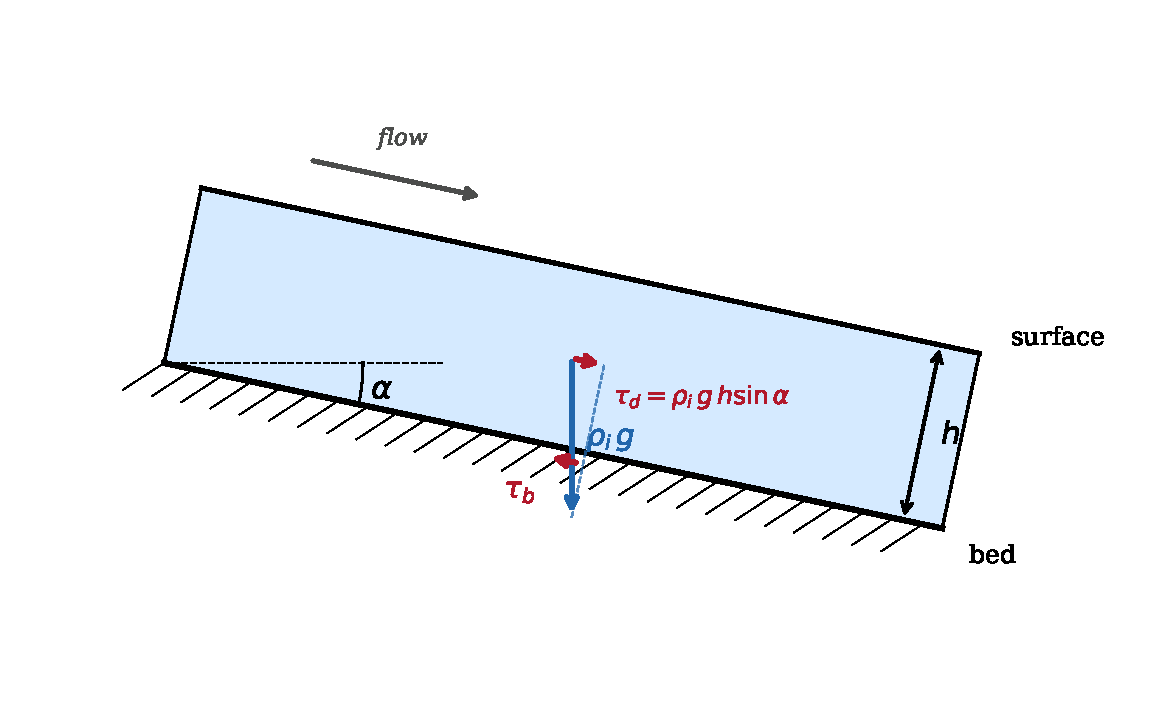
\includegraphics[width=0.75\textwidth]{figures/fig00_parallel_slab_schematic.pdf}
  \caption{Parallel-slab geometry.  A uniform slab of ice with thickness $h$ rests on a bed inclined at angle $\alpha$.  The free body extends from the surface down to depth $d = s - z$: the downslope gravity component $\rho_i g d \sin\alpha$ is balanced by the shear traction $|\tau_{xz}(z)|$ on the base of the block.}
  \label{fig:slab_schematic}
\end{figure}

\subsection{Stress Distribution from a Free-Body Diagram}

Consider a block of ice extending from the free surface ($z = s$) down to some level $z$ within the ice.  The block has thickness $d = s - z$ and unit horizontal and lateral extent.

\medskip
\noindent The forces acting on this block per unit area are:
\begin{itemize}
  \item \textbf{Gravity component along the slope:} $\rho_i g\,d\,\sin\alpha$ (downslope).
  \item \textbf{Shear traction on the base of the block:} $|\tau_{xz}(z)|$ (opposing motion, upslope).
  \item \textbf{Tractions on the surface:} zero (free surface).
\end{itemize}

\noindent Balancing forces in the downslope ($+x$) direction.  The gravity component is $\rho_i g\,d\,\sin\alpha$ (downslope).  The shear traction on the base of the block, exerted by the ice below on the face with outward normal $-\hat{z}$, is $-\tau_{xz}$ (the minus sign from the outward normal).  Setting the net force to zero:
\begin{equation}
  \rho_i g\,(s - z)\,\sin\alpha - \tau_{xz}(z) = 0,
\end{equation}
so:
\begin{equation}
  \boxed{\tau_{xz}(z) = \rho_i g\,(s - z)\,\sin\alpha.}
  \label{eq:slab_stress}
\end{equation}
The shear stress is positive: ice above height $z$ is driven downslope by gravity, and the resulting viscous coupling means faster-moving ice above drags slower-moving ice below.  The stress increases linearly from zero at the surface to a maximum at the bed:
\begin{equation}
  \tau_b \equiv \tau_{xz}(b) = \rho_i g\,h\,\sin\alpha.
  \label{eq:basal_shear}
\end{equation}
For small slopes ($\sin\alpha \approx \tan\alpha = -\partial s/\partial x$), the basal shear stress equals the driving stress:
\begin{equation}
  \tau_b = \rho_i g\,h\,\sin\alpha \approx -\rho_i g\,h\,\frac{\partial s}{\partial x} = \tau_d,
\end{equation}
recovering the expression from the stress lecture.

\medskip
\noindent\emph{Note:} We have derived this stress distribution from a simple force balance on a block of ice.  This is a special case of the general conservation of linear momentum, which we will introduce formally in a later lecture.  The key simplification here is that $\partial/\partial x = 0$ eliminates all terms involving longitudinal and lateral stress gradients.

\subsection{Velocity Profile}
\label{sec:velocity_profile}

\begin{tcolorbox}[
  colback=orange!25,
  colframe=orange!70!black,
  title={\textbf{Derivation: Velocity Profile for Simple Shear}},
  breakable
]
With only $\tau_{xz}$ nonzero, the effective stress simplifies to $\tau_e = \tau_{xz}$ (which is positive).  Glen's flow law~\eqref{eq:glen} gives:
\begin{equation}
  \dot{\varepsilon}_{xz} = A\,\tau_{xz}^{n-1}\,\tau_{xz} = A\,\tau_{xz}^n.
\end{equation}
Since $\partial w/\partial x = 0$ for the parallel slab, the shear strain rate is $\dot{\varepsilon}_{xz} = \frac{1}{2}\partial u/\partial z$, so:
\begin{equation}
  \frac{\partial u}{\partial z} = 2A\,\bigl(\rho_i g \sin\alpha\bigr)^n\,(s - z)^n.
  \label{eq:dudzraw}
\end{equation}

\noindent Integrating from the bed ($z = b$, where $u = u_b$) to height $z$.  Let $\zeta = s - z'$ so that $d\zeta = -dz'$:
\begin{align}
  u(z) - u_b &= \int_b^z 2A\,(\rho_i g \sin\alpha)^n (s - z')^n\,dz' \notag\\[4pt]
  &= 2A\,(\rho_i g \sin\alpha)^n \left[-\frac{(s-z')^{n+1}}{n+1}\right]_b^z \notag\\[4pt]
  &= \frac{2A}{n+1}\,(\rho_i g \sin\alpha)^n \left[h^{n+1} - (s - z)^{n+1}\right].
\end{align}

\medskip
\noindent The velocity at any height $z$ above the bed is therefore
\begin{equation}
  \boxed{u(z) = u_b + \frac{2A}{n+1}\,(\rho_i g \sin\alpha)^n \left[h^{n+1} - (s - z)^{n+1}\right],}
  \label{eq:velocity_profile}
\end{equation}
where $u_b$ is the basal sliding velocity (prescribed as a boundary condition; for now we set $u_b = 0$).

\medskip
\noindent The surface velocity (at $z = s$) is:
\begin{equation}
  u_s = u_b + \frac{2A}{n+1}\,(\rho_i g \sin\alpha)^n\,h^{n+1}.
  \label{eq:surface_vel}
\end{equation}
The velocity due to internal deformation scales as $\tau_d^n\,h$, or equivalently as $h^{n+1}$ for fixed surface slope.  For $n = 3$, the deformational velocity depends on the \emph{fourth power} of the ice thickness---a very strong sensitivity.
\end{tcolorbox}

\subsection{Shape of the Velocity Profile}

Figure~\ref{fig:velocity_profiles} shows normalized velocity profiles for several values of $n$.  The key observation is that deformation is \textbf{concentrated near the bed}.  Writing $u(z)/u_s$ as a function of the normalized height $\hat{z} = (z - b)/h$:
\begin{equation}
  \frac{u(z)}{u_s} = 1 - (1 - \hat{z})^{n+1}.
  \label{eq:normalized_profile}
\end{equation}

\begin{figure}[ht]
  \centering
  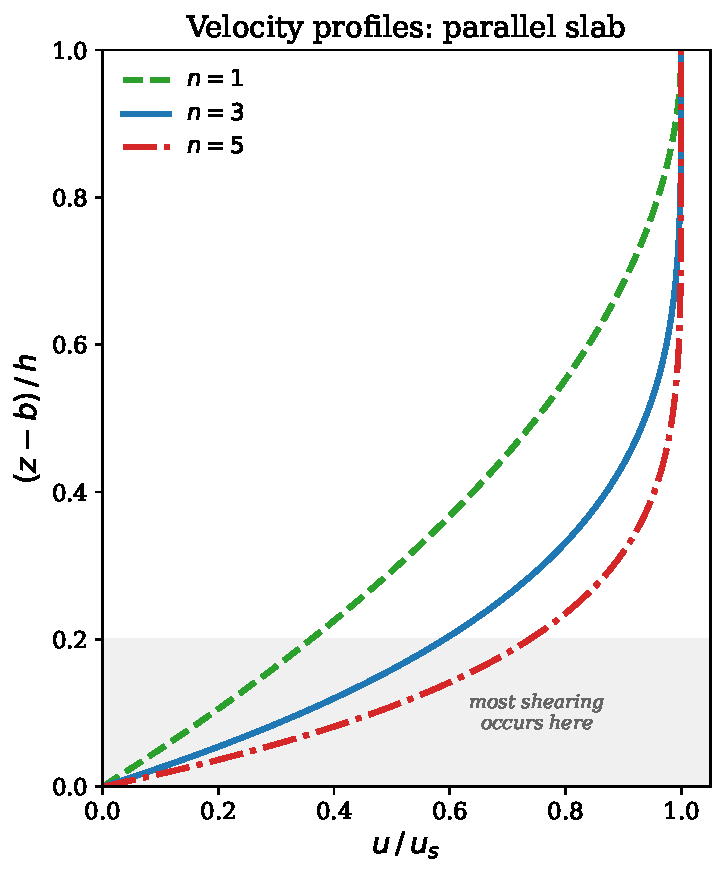
\includegraphics[width=0.6\textwidth]{figures/fig01_velocity_profiles.pdf}
  \caption{Normalized velocity profiles $u/u_s$ vs.\ height above bed $(z-b)/h$ for the parallel-slab problem with $n = 1$ (Newtonian), $n = 3$ (standard Glen's law), and $n = 5$.  For $n = 3$, roughly 80\% of the surface velocity is achieved in the upper half of the ice column; most shearing occurs in the basal 20\%.}
  \label{fig:velocity_profiles}
\end{figure}

\noindent For $n = 1$ (Newtonian fluid), the profile is parabolic.  For $n = 3$, the upper $\sim$80\% of the ice column moves nearly as a rigid ``plug,'' with intense shearing confined to the basal $\sim$20\%.  As $n$ increases, the profile becomes increasingly plug-like, approaching a perfectly plastic limit in which all deformation occurs in a thin basal layer.

\subsection{Depth-Averaged Velocity and Flux}

The depth-averaged velocity is:
\begin{equation}
  \bar{u} = \frac{1}{h}\int_b^s u(z)\,dz = u_b + \frac{2A}{n+2}\,(\rho_i g \sin\alpha)^n\,h^{n+1}.
\end{equation}
The ratio of the depth-averaged to the surface deformational velocity is:
\begin{equation}
  \frac{\bar{u} - u_b}{u_s - u_b} = \frac{n + 1}{n + 2}.
  \label{eq:ubar_ratio}
\end{equation}
For $n = 3$: $\bar{u} = u_b + \tfrac{4}{5}(u_s - u_b)$.

\medskip
\noindent The depth-integrated \textbf{flux per unit width} is:
\begin{equation}
  \boxed{q = \bar{u}\,h = u_b\,h + \frac{2A}{n+2}\,(\rho_i g \sin\alpha)^n\,h^{n+2}.}
  \label{eq:flux_slab}
\end{equation}
This is the expression that will enter the continuity equation to determine ice sheet profiles.  Note the strong dependence on thickness: $q \propto h^{n+2}$ for the deformational part (i.e., $q \propto h^5$ for $n = 3$).

% CHALKBOARD DRAWING 4:
% Draw the velocity profile for n = 3.
% Mark u_s, u_bar, and shade the area between u(z) and zero to represent the flux q.
% Annotate: "most shearing here" near the bed, "plug-like flow" in the upper part.

\medskip
\noindent\textbf{Two end-member flow regimes:}
\begin{itemize}
  \item $u_b = 0$: all motion is from internal deformation (frozen bed).  This is the regime we focus on for deriving ice sheet profiles.
  \item $u_b \gg u_s - u_b$: sliding dominates and the flow is approximately plug-like.  This regime characterizes ice streams.
\end{itemize}

%===================================================================
% SECTION 5 -- Ice Sheet as a Viscous Gravity Current
%===================================================================
\section{The Ice Sheet as a Viscous Gravity Current}
\label{sec:gravity_current}

We now use the slab solution to compute the surface profile of a two-dimensional ice sheet in steady state.  The idea is simple: if the ice sheet is much wider than it is thick, then the flow at any point is well approximated by the local slab solution.

\subsection{The Shallow-Ice Approximation}

A typical large ice sheet has a thickness of $h \sim 3$~km and a half-span of $L \sim 1000$~km, giving an aspect ratio
\begin{equation}
  \varepsilon = \frac{[h]}{[L]} \sim 3 \times 10^{-3}.
\end{equation}
When $\varepsilon \ll 1$, a scaling analysis of the full stress-balance equations (which we will develop in a later lecture) shows that:
\begin{itemize}
  \item The dominant stress is the vertical shear stress $\tau_{xz}$.
  \item Longitudinal deviatoric stresses ($\tau_{xx}$) are smaller by a factor of $O(\varepsilon^2)$.
  \item The pressure is approximately glaciostatic.
\end{itemize}
Under these conditions, the ice at each location deforms as though it were part of a parallel slab with the local thickness and surface slope.  This is the \textbf{shallow-ice approximation} (SIA).

% CHALKBOARD DRAWING 5:
% Sketch a cross-section of an ice sheet with greatly exaggerated vertical scale.
% Show that at each column, the local slab solution applies.
% Annotate: "each column sees only local h and ds/dx."

\subsection{The SIA Flux}

Under the SIA with no basal sliding and a flat bed ($s = h$), the flux from Eq.~\eqref{eq:flux_slab} becomes:
\begin{equation}
  q(x) = -\frac{2A}{n+2}\,(\rho_i g)^n\,\left|\frac{\partial s}{\partial x}\right|^{n-1}\frac{\partial s}{\partial x}\;h^{n+2},
  \label{eq:SIA_flux}
\end{equation}
where the sign ensures that flux is in the direction of decreasing surface elevation.  Substituting $s = h$ (flat bed):
\begin{equation}
  q(x) = -\frac{2A}{n+2}\,(\rho_i g)^n\,\left|\frac{dh}{dx}\right|^{n-1}\frac{dh}{dx}\;h^{n+2}.
  \label{eq:SIA_flux_flat}
\end{equation}

\subsection{Coupling to the Continuity Equation}

The vertically integrated continuity equation at steady state is:
\begin{equation}
  \dot{b}_i = \frac{dq}{dx}.
  \label{eq:steady_continuity}
\end{equation}
Substituting the SIA flux~\eqref{eq:SIA_flux_flat} yields a nonlinear ordinary differential equation for $h(x)$.  In full generality this must be solved numerically, but for uniform accumulation on a flat bed, an analytical solution exists.

\subsection{The Vialov Profile}
\label{sec:vialov}

\begin{tcolorbox}[
  colback=orange!25,
  colframe=orange!70!black,
  title={\textbf{Derivation: The Vialov Profile}},
  breakable
]

\textbf{Setup.}  Consider a symmetric ice sheet on a flat, horizontal bed with uniform accumulation rate $\dot{b}_i > 0$ and no basal sliding.  Place the origin at the ice divide; the margin is at $x = L$ (half-span).  By symmetry, $q(0) = 0$ and $dh/dx\big|_{x=0} = 0$.

\medskip
\noindent\textbf{Step 1: Integrate the continuity equation.}

From Eq.~\eqref{eq:steady_continuity}, integrating from the divide:
\begin{equation}
  q(x) = \dot{b}_i\,x.
  \label{eq:flux_linear}
\end{equation}
The flux increases linearly from zero at the divide to $\dot{b}_i L$ at the margin.

\medskip
\noindent\textbf{Step 2: Equate with the SIA flux.}

Using $q > 0$ for $x > 0$ (flow toward the margin, $dh/dx < 0$):
\begin{equation}
  \frac{2A}{n+2}\,(\rho_i g)^n\,\left(-\frac{dh}{dx}\right)^n h^{n+2} = \dot{b}_i\,x.
  \label{eq:vialov_ode}
\end{equation}

\medskip
\noindent\textbf{Step 3: Separate variables and integrate.}

Rearranging and writing $\left(-dh/dx\right)^n = \dot{b}_i x \cdot (n+2) / [2A\,(\rho_i g)^n\,h^{n+2}]$, then integrating with the boundary condition $h(L) = 0$, the solution is:

\begin{equation}
  \boxed{h(x) = h_0 \left[1 - \left(\frac{x}{L}\right)^{\frac{n+1}{n}}\right]^{\frac{n}{2(n+1)}},}
  \label{eq:vialov}
\end{equation}
where the divide thickness is
\begin{equation}
  \boxed{h_0 = \left[\frac{2^{n-1}(n+2)\,\dot{b}_i}{A\,(\rho_i g)^n}\right]^{1/(2n+2)} L^{(n+1)/(2n+2)}.}
  \label{eq:vialov_h0}
\end{equation}
\end{tcolorbox}

\begin{figure}[ht]
  \centering
  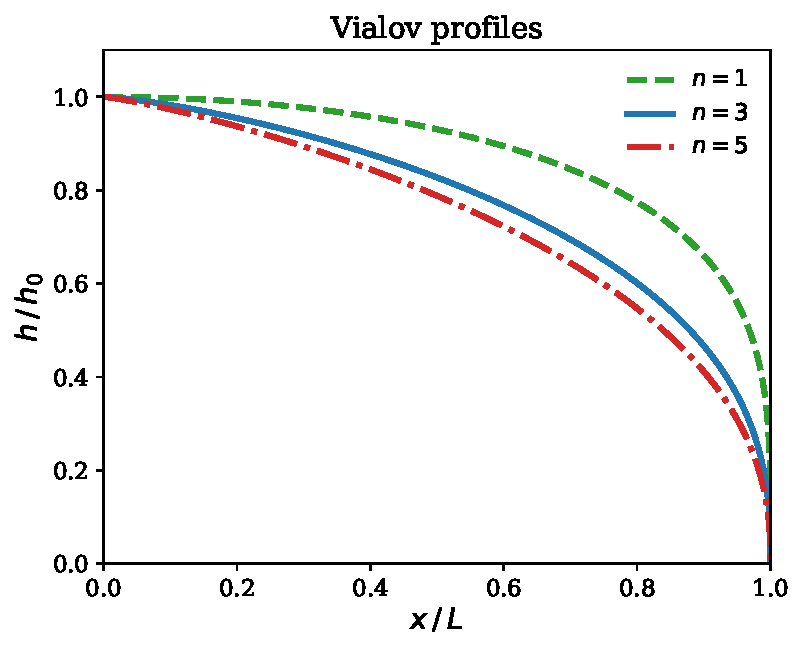
\includegraphics[width=0.65\textwidth]{figures/fig02_vialov_profiles_n.pdf}
  \caption{Normalized Vialov profiles $h/h_0$ vs.\ $x/L$ for $n = 1$, $3$, and~$5$.  Higher $n$ produces steeper margins and a flatter interior, reflecting the increasing concentration of deformation in high-stress regions.}
  \label{fig:vialov_n}
\end{figure}

\subsection{Insensitivity to Parameters}
\label{sec:insensitivity}

A remarkable feature of the Vialov solution is the \textbf{weak dependence} of $h_0$ on both the accumulation rate and the rate factor:
\begin{equation}
  h_0 \propto \left(\frac{\dot{b}_i}{A}\right)^{1/(2n+2)}.
\end{equation}
For $n = 3$, the exponent is $1/8 = 0.125$.  Consequences:
\begin{itemize}
  \item \textbf{Doubling} $\dot{b}_i$ increases $h_0$ by only $\sim\!9$\%.
  \item An \textbf{eight-fold} change in $\dot{b}_i$ changes $h_0$ by $\sim\!30$\%.
  \item The same insensitivity holds for $A$, meaning that large uncertainties in the rate factor have a modest effect on the predicted profile.
\end{itemize}
Ice sheet shape is set primarily by the span $L$ and by gravity; the rheological and climate details enter only weakly.  This is a direct consequence of the nonlinearity of Glen's law: the strong dependence of flux on thickness ($q \propto h^{n+2}$) acts as a powerful negative feedback that limits thickness variations.

\begin{figure}[ht]
  \centering
  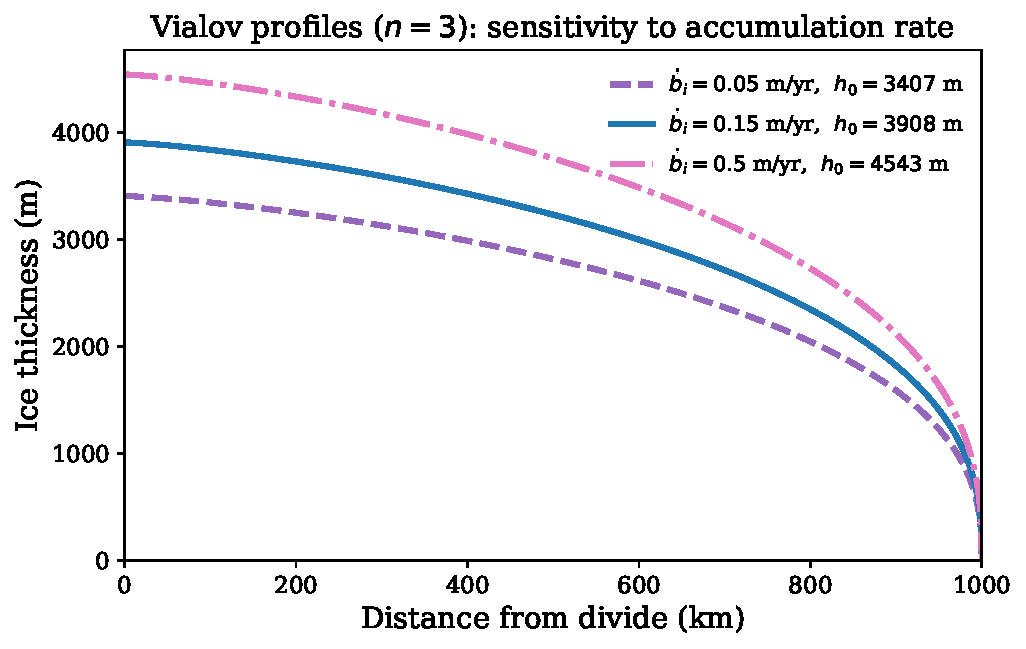
\includegraphics[width=0.65\textwidth]{figures/fig03_vialov_insensitivity.pdf}
  \caption{Vialov profiles ($n = 3$) for accumulation rates spanning an order of magnitude.  Despite large differences in $\dot{b}_i$, the profiles are strikingly similar.}
  \label{fig:vialov_sensitivity}
\end{figure}

%===================================================================
% SECTION 6 -- Perfectly Plastic Limit
%===================================================================
\section{The Perfectly Plastic Limit}
\label{sec:plastic}

An instructive limiting case is obtained by taking $n \to \infty$ in Glen's law.  In this limit, ice behaves as a \textbf{perfectly plastic material}: it does not deform at all below a yield stress $\tau_0$, and it flows freely at stress equal to $\tau_0$.

\medskip
\noindent If the basal shear stress equals the yield stress everywhere, the force balance gives:
\begin{equation}
  \rho_i g\,h\left|\frac{dh}{dx}\right| = \tau_0.
  \label{eq:plastic_ode}
\end{equation}
Separating variables:
\begin{equation}
  h\,dh = -\frac{\tau_0}{\rho_i g}\,dx,
\end{equation}
where the sign accounts for $dh/dx < 0$ (surface slopes downward from divide to margin).  Integrating from the margin ($x = L$, $h = 0$) inward:

\begin{equation}
  \boxed{h^2(x) = \frac{2\tau_0}{\rho_i g}\,(L - x).}
  \label{eq:parabolic}
\end{equation}
This is a \textbf{parabolic profile}, first derived by \cite{Nye1952}.  The divide thickness is:
\begin{equation}
  h_0 = \sqrt{\frac{2\tau_0 L}{\rho_i g}}.
  \label{eq:plastic_h0}
\end{equation}

\noindent With $\tau_0 \approx 100$~kPa, $L = 1000$~km, and $\rho_i g \approx 9000$~N\,m$^{-3}$:
\begin{equation}
  h_0 = \sqrt{\frac{2 \times 10^5 \times 10^6}{9 \times 10^3}} \approx 4700~\text{m},
\end{equation}
which is in the right ballpark for a large ice sheet (the East Antarctic ice sheet has a divide thickness of $\sim$4000~m for a comparable half-span), though the agreement is best when a more realistic yield stress is chosen.

\begin{figure}[ht]
  \centering
  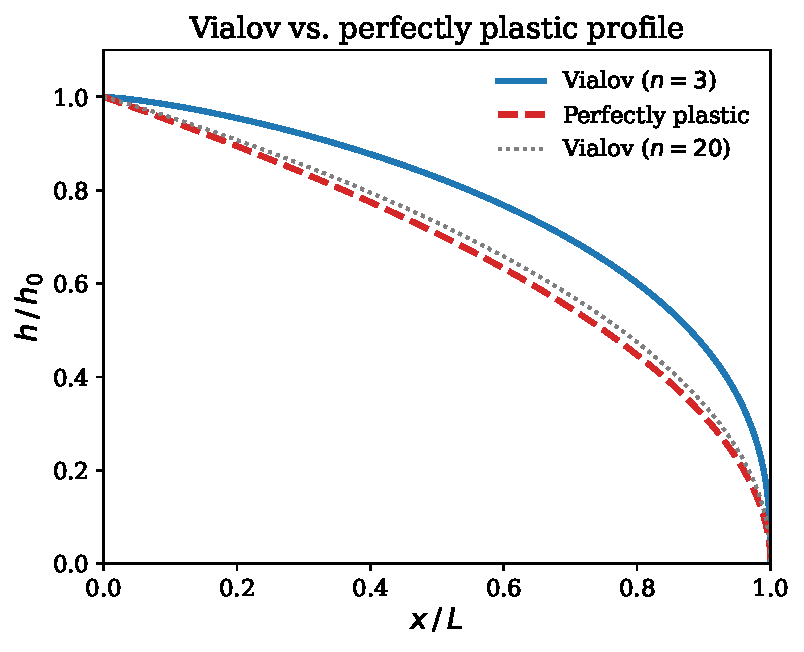
\includegraphics[width=0.65\textwidth]{figures/fig04_plastic_vs_vialov.pdf}
  \caption{Comparison of the Vialov profile ($n = 3$) with the perfectly plastic (parabolic) profile.  The two are remarkably similar: flat in the interior, steep at the margins.  The plastic profile slightly overestimates thickness near the divide and underestimates it near the margins.}
  \label{fig:plastic_vs_vialov}
\end{figure}

\noindent The resemblance between the Vialov and parabolic profiles (Fig.~\ref{fig:plastic_vs_vialov}) is striking.  Both share the same qualitative features:
\begin{itemize}
  \item Flat interior (small surface slopes near the divide).
  \item Steep margins (large slopes as $h \to 0$).
  \item Divide thickness that scales as $\sqrt{L}$.
\end{itemize}
This similarity reinforces the conclusion that ice sheet shape is controlled primarily by the geometry and gravity, not by the details of the rheology.

%===================================================================
% SECTION 7 -- Comparison with Observations
%===================================================================
\section{Comparison with Observations}
\label{sec:observations}

How well do these idealized profiles match real ice sheets?  Figure~\ref{fig:observed} compares the Vialov and plastic profiles with a representative transect across the East Antarctic ice sheet.

\begin{figure}[ht]
  \centering
  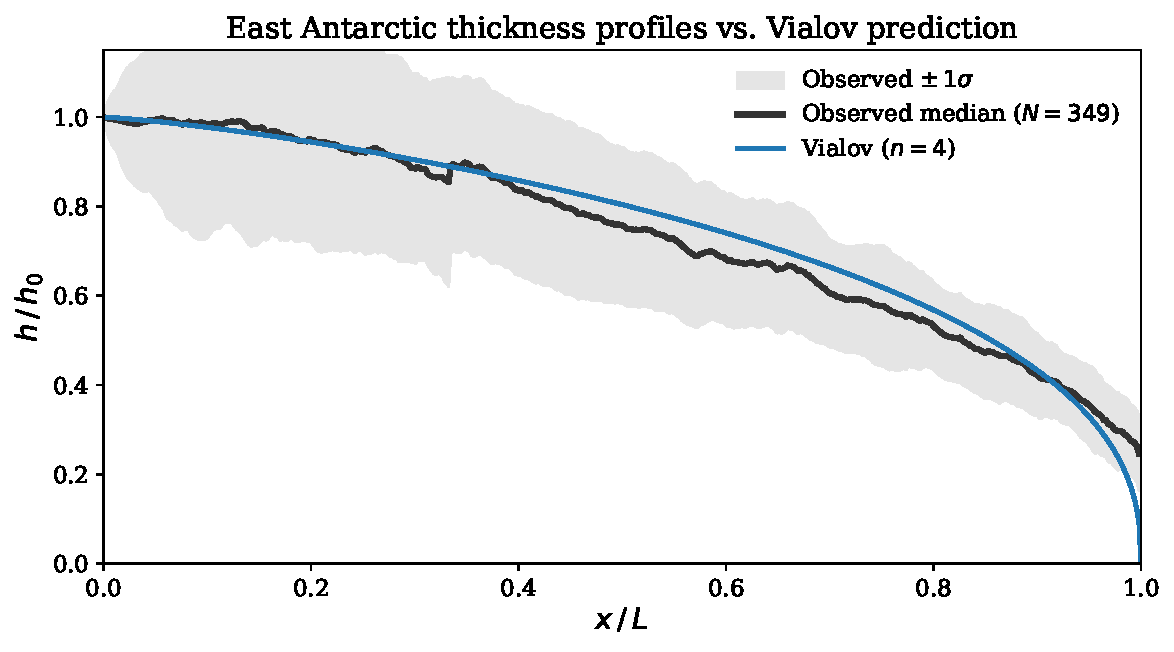
\includegraphics[width=0.7\textwidth]{figures/fig05_observed_vs_predicted.pdf}
  \caption{Normalized ice thickness profiles along 349 flowlines in East Antarctica (BedMachine Antarctica v4.1; \cite{Morlighem2020}) compared with the Vialov profile for $n = 4$.  Flowlines were seeded in fast-flowing ice and traced upstream to the divide; only profiles reaching the ridge are shown.  For each profile, the Vialov half-span $L$ was fitted to minimize the RMS misfit at $n = 4$ (which fits marginally better than $n = 3$), and thickness is normalized by the divide value $h_0$.  The dark line shows the observed median; the shaded band is $\pm 1$ standard deviation.  The Vialov prediction captures the interior profile shape well but overpredicts thickness near the margins, where basal sliding and ice stream dynamics --- not captured by the SIA --- become important.}
  \label{fig:observed}
\end{figure}

\medskip
\noindent\textbf{Interior ($|x| \lesssim 0.7L$):}  The agreement is generally good.  In the slow-flowing interior, the bed is often frozen, basal sliding is negligible, and the SIA assumptions are well satisfied.

\medskip
\noindent\textbf{Margins ($|x| \gtrsim 0.7L$):}  The predicted profiles systematically deviate from observations.  The ice is typically thinner and the surface steeper than predicted.  Several mechanisms contribute:

\begin{enumerate}
  \item \textbf{Basal sliding.}  The models assume $u_b = 0$.  Near the margins, the bed is often at the pressure melting point, and sliding can be the dominant component of velocity.  Sliding evacuates ice more efficiently, producing a thinner profile.

  \item \textbf{Ice streams and outlet glaciers.}  Fast-flowing features violate the SIA because longitudinal stress gradients and lateral drag are dynamically important.  The flow is no longer controlled by local thickness and slope alone.

  \item \textbf{Temperature variations.}  The rate factor $A$ increases with temperature.  Since ice near the margins is generally warmer (due to both surface climate and strain heating), the ice there is effectively softer than assumed by a uniform $A$.

  \item \textbf{Non-uniform accumulation.}  Accumulation rates are not spatially uniform; they tend to decrease with distance from the coast (orographic effects) and vary with elevation.

  \item \textbf{Marine-terminating margins.}  Many Antarctic outlet glaciers terminate in the ocean, where the dynamics of calving, buttressing by ice shelves, and ocean-induced basal melting govern the margin position---none of which is captured by the simple models.
\end{enumerate}

\noindent The systematic pattern of failure at the margins is informative: it tells us precisely which physical processes we need to incorporate to build more complete models.  The full conservation of linear momentum---and the richer dynamics it permits---is the subject of subsequent lectures.

%===================================================================
% SECTION 8 -- Summary
%===================================================================
\section{Summary}

Key results from this lecture:

\begin{enumerate}
  \item \textbf{The strain-rate tensor} $\dot{\varepsilon}_{ij}$ measures the rate of deformation.  It is the symmetric part of the velocity gradient tensor.  Incompressibility requires $\dot{\varepsilon}_{kk} = 0$.

  \item \textbf{Glen's flow law} $\dot{\varepsilon}_{ij} = A\,\tau_e^{n-1}\,\tau_{ij}$ with $n \approx 3$ is the constitutive relation for glacier ice.  It implies shear-thinning: deformation concentrates where stress is large.

  \item \textbf{The parallel-slab solution} gives the velocity profile under simple shear:
  \begin{equation*}
    u(z) = u_b + \frac{2A}{n+1}(\rho_i g \sin\alpha)^n \left[h^{n+1} - (s-z)^{n+1}\right].
  \end{equation*}
  For $n = 3$, most shearing occurs in the basal $\sim$20\% of the ice column.

  \item \textbf{The shallow-ice approximation} treats each column as a local slab, coupling the flux $q \propto h^{n+2}|ds/dx|^{n-1}(ds/dx)$ to the continuity equation.

  \item \textbf{The Vialov profile} gives the steady-state surface elevation of an ice sheet.  Divide thickness depends on accumulation and the rate factor only through $(\dot{b}_i/A)^{1/8}$---an extraordinary insensitivity that reflects the strong nonlinearity of the flux--thickness relation.

  \item \textbf{The perfectly plastic profile} ($n \to \infty$) is a parabola, $h^2 \propto (L - x)$, and is strikingly similar to the Vialov profile.  Ice sheet shape is dominated by geometry and gravity.

  \item \textbf{Where the SIA fails}---at the margins, in ice streams, and at marine-terminating outlets---tells us what physics must come next: basal sliding, longitudinal stress gradients, lateral drag, and ocean--ice interaction.
\end{enumerate}

%===================================================================
% Reading
%===================================================================
\section*{Reading}

Cuffey \& Paterson, \textit{Physics of Glaciers}, 4th ed.:
\begin{itemize}
  \item Section 3.4: Overview of the flow law (preview for later lectures)
  \item Sections 8.2--8.3: Strain rates and the velocity gradient tensor
  \item Sections 8.5.1--8.5.3: Glen's flow law and effective viscosity
  \item Section 9.3: Parallel-flow solutions (slab on a slope)
  \item Section 9.4: Steady-state profiles of ice sheets (Vialov)
  \item Section 9.5.1: Perfectly plastic glaciers
\end{itemize}

%===================================================================
% Bibliography
%===================================================================
\begin{thebibliography}{99}

\bibitem{Glen1955}
Glen, J.~W.\ (1955).
The creep of polycrystalline ice.
\textit{Proceedings of the Royal Society of London.\ Series A}, 228(1175), 519--538.
\texttt{doi:10.1098/rspa.1955.0066}

\bibitem{Morlighem2020}
Morlighem, M., et~al.\ (2020).
Deep glacial troughs and stabilizing ridges unveiled beneath the margins of the Antarctic ice sheet.
\textit{Nature Geoscience}, 13, 132--137.
\texttt{doi:10.1038/s41561-019-0510-8}

\bibitem{Hutter1983}
Hutter, K.\ (1983).
\textit{Theoretical Glaciology: Material Science of Ice and the Mechanics of Glaciers and Ice Sheets}.
D.\ Reidel Publishing Company.
\texttt{doi:10.1007/978-94-015-1167-4}

\bibitem{Nye1952}
Nye, J.~F.\ (1952).
The mechanics of glacier flow.
\textit{Journal of Glaciology}, 2(12), 82--93.
\texttt{doi:10.3189/S0022143000033967}

\bibitem{Nye1957}
Nye, J.~F.\ (1957).
The distribution of stress and velocity in glaciers and ice-sheets.
\textit{Proceedings of the Royal Society of London.\ Series A}, 239(1216), 113--133.
\texttt{doi:10.1098/rspa.1957.0026}

\bibitem{Vialov1958}
Vialov, S.~S.\ (1958).
Regularities of glacial shields movement and the theory of plastic viscous flow.
\textit{International Association of Hydrological Sciences Publication}, 47, 266--275.

\end{thebibliography}

\end{document}
